\chapter{Parameter Inference}

\section{Motivation}

Building mathematical models of real-world phenomena allows us to
simulate changes in the world without undertaking large-scale
experiments. However, once we have a model that sufficiently approximates
\emph{P. vivax} transmission
or anything else we are trying to model,
we need to estimate the `true' underlying parameters.
We calibrate the model against real-world data such as case counts
and prevalence surveys to do this. 
Under frequentist assumptions, there is a `true' set of
parameters that simulated the observed data. In the Bayesian
framework, the parameters are considered to be random, and
This chapter explores statistical inference techniques to recover the
parameters under both the frequentist and Bayesian frameworks.

\section{Frequentist Parameter Estimation}

Assume the model is parameterised by a set of parameters
$\btheta \in \mathbf{\Theta},$ which
we are trying to estimate by considering some observed data
$\by^\obs = (y_1^\obs, \dots, y_n^\obs).$
Consider $\by(\btheta) = (y_1(\btheta), \dots, y_n(\btheta))$
some model simulation of
$\by^\obs.$ Often, the observed data has some underlying index set
$x_1, \dots, x_n,$ where $x_i$ might be something like time. In this case,
we can also consider the observed data to be
$\{(x_1, y_1^\obs), \dots, (x_n, y_n^\obs)\},$ and the
model simulated data to be
$\{(x_1, y_1(\btheta)), \dots, (x_n, y_n(\btheta))\}.$

\subsection*{Least Squares Estimator}

It is common for models to be deterministic, for example, when
modelling the mean behaviour
of a system. In this case, $\by(\btheta)$ is not random. Therefore,
we can assume that $y^\obs_i = y_i(\btheta) + \varepsilon_i,$
where $\varepsilon_i$ is a random variable with some (possibly unknown)
distribution and zero mean.

When the distribution of $\varepsilon_i$ is unknown, a common approach for
estimating $\btheta^{\LS}$ is to take the least squares estimate
(although we show in Theorem \ref{thm:LSE_normal} that implicitly normal noise
is assumed).

\begin{definition}[Least Squares Estimate]
    The \bemph{least squares estimate} $\btheta^{\LS}$ for
    $\btheta$ is
    $$
        \btheta^{\LS}
        := \argmin_{\btheta\in\mathbf{\Theta}}
        \sum_{i = 1}^n (y_i(\btheta)- y_i^\obs)^2.
    $$
\end{definition}

\begin{example}\label{ex:LSE}
    Consider the observed data
    $\{(x_1, y_1^\obs), (x_2, y_2^\obs), (x_3, y_3^\obs)\}
        = \{(1, 2), (2, 4), (3, 4)\},$
    which we assume were generated from the model
    $y_i(\btheta) + \varepsilon_i.$ Let
    $y_i(\btheta) = \theta_0 + \theta_1x_i$ and
    $\E(\varepsilon_i) = 0.$ We derive the least squares estimate of our
    parameters $\btheta = (\theta_0, \theta_1)$ by

    \begin{align*}
        \btheta^{\LS}
        = & \, \argmin_{\btheta}
        [\sum_{i = 1}^3 (y_i(\btheta) - y_i^\obs)^2]           \\
        = & \, \argmin_{\btheta}
        [\sum_{i = 1}^3 (\theta_0 + \theta_1x_i - y_i^\obs)^2] \\
        = & \, \argmin_{\btheta}
        [(\theta_0 + \theta_1 - 2)^2 + (\theta_0 + 2\theta_1 - 4)^2
            + (\theta_0 + 3\theta_1 - 4)^2].
    \end{align*}

    Since the expanded quadratic will have positive coefficients for
    $\theta_0$ and $\theta_1,$ we can solve for $\btheta^{\LS}$
    by
    \begin{align*}
        \mathbf{0}
        = & \, \frac{\partial}{\partial \btheta}
        [
            (\theta^\LS_0 + \theta^\LS_1 - 2)^2
            + (\theta^\LS_0 + 2\theta^\LS_1 - 4)^2
            + (\theta^\LS_0 + 3\theta^\LS_1 - 4)^2
        ]                                        \\
        = & \begin{bmatrix}
                6\theta^\LS_0 + 12\theta^\LS_1 - 20 \\
                12\theta^\LS_0 + 28\theta^\LS_1 - 44
            \end{bmatrix}.
    \end{align*}

    Solving these two equations results in $\theta^\LS_0 = 4/3$ and
    $\theta^\LS_1 = 1.$ This can be visually seen in Figure \ref{fig:LSE} in
    the red line that minimises the sum of the squares of the difference
    between the observations (in black dots) and the linear model.
\end{example}


\begin{figure}[htbp]
    \centering
    \includegraphics[width=\textwidth]{LS_example.pdf}
    \caption[{
        Maximum likelihood and least squares linear regression examples
    }]{
        Two linear models of the form
        $y_i(\btheta) = \theta_0 + \theta_1x_i$ fit given the set
        of observations $\{(1, 2), (2, 4), (3, 4)\}$ using the method of
        least squares and maximum likelihood under
        the assumption that the data are independent realisations from a Poisson
        distribution with mean $y_i(\btheta).$ The least squares estimates
        were $\theta^\LS_0 = 4/3$ and $\theta^\LS_1 = 1.$ The maximum likelihood
        estimates were $\hat{\theta}_0 \approx 1.329$ and
        $\hat{\theta}_1 \approx 0.751.$
    }
    \label{fig:LSE}
\end{figure}

\subsection*{Maximum Likelihood Estimator}

The least squares method makes no explicit assumptions about the distribution
of the noise $\varepsilon.$ However, if the distribution of $\varepsilon$ is
known (or can be reasonably assumed), we can
explicitly calculate the probability of the data given the parameters.

\begin{definition}[Likelihood function]
    With $\by^\obs$ fixed, the \bemph{likelihood function} is
    $$
        \mathcal{L}(\btheta)
        := \Pr(
        \by(\btheta) + \bm{\varepsilon} = \by^\obs
        | \btheta
        ).
    $$
    Particularly, if $y_i(\btheta) + \varepsilon_i$ are independent
    $$
        \mathcal{L}(\btheta)
        = \prod_{i = 1}^n
        \Pr(
        y_i(\btheta) + \varepsilon_i = y_i^\obs
        | \btheta
        ).
    $$
\end{definition}

The dependence of the likelihood function on $\by^\obs$ is notationally
suppressed but can be
explicitly written as $\mathcal{L}(\btheta|\by^\obs)$ to avoid confusion.
In the continuous
(or mixture of discrete and continuous) case,
we interpret
$
    \Pr(
    \by(\btheta) + \bm{\varepsilon} = \by^\obs
    | \btheta
    )
$
as the density
$
    \Pr(
    \by(\btheta) + \bm{\varepsilon} \in \diff\by^\obs
    | \btheta
    )
$ with respect to an underlying probability measure.

A natural estimate for $\btheta$ is the one that maximises the likelihood
function $\mathcal{L}$, as it coincides with the value of $\btheta$
that maximises the
probability of the data (possibly expressed as a density).
Such an estimate is called the maximum likelihood
estimate.

\begin{definition}[Maximum Likelihood Estimate]
    The \bemph{maximum likelihood estimate} of $\btheta$ is
    $$
        \hat{\btheta}
        := \argmax_{\btheta\in\mathbf{\Theta}} \mathcal{L}(\btheta).
    $$
\end{definition}

It is often computationally easier to deal with the log-likelihood
$\ell(\btheta) := \ln\mathcal{L}(\btheta).$ Since the natural
logarithm is a monotonic function,
$$
    \argmax_{\btheta\in\mathbf{\Theta}} \mathcal{L}(\btheta)
    = \argmax_{\btheta\in\mathbf{\Theta}} \ell(\btheta).
$$

\begin{example}
    Using the same observed data set as Example \ref{ex:LSE}, we assume that
    $y_i^\obs$ were generated independently from
    $y_i(\btheta) + \varepsilon_i \sim \Pois(y_i(\btheta)),$ where
    $y_i(\btheta) := \theta_0 + \theta_1x_i$ as previously defined. Therefore,
    the maximum likelihood estimate of $\btheta$ is
    \begin{align*}
        \hat{\btheta}
        = & \, \argmax \ell(\btheta)                                  \\
        = & \, \argmax_{\btheta\in\mathbf{\Theta}}\sum_{i = 1}^{3}
        y_i^\obs\ln(y_i(\btheta)) -y_i^\obs(\btheta) - \ln(y_i^\obs!) \\
        = & \, \argmax_{\btheta\in\mathbf{\Theta}}\sum_{i = 1}^{3}
        y_i^\obs\ln(\theta_0 + \theta_1x_i)
        - \theta_0 - \theta_1x_i
        - \ln(y_i^\obs!)                                              \\
        = & \, \argmax_{\btheta\in\mathbf{\Theta}}
        2\ln(\theta_0 + \theta_1) - \theta_0 - \theta_1
        + 4\ln(\theta_0 + 2\theta_1) - \theta_0 - 2\theta_1
        + 4\ln(\theta_0 + 3\theta_1) - \theta_0 - 3\theta_1.
    \end{align*}
    
    Numerically solving, we obtain $\hat{\theta}_0 \approx 1.329,$
    and $\hat{\theta_1} \approx 0.751,$ as seen by the green line in Figure 
    \ref{fig:LSE}. This estimate is not the same as the linear model
    estimate using the least squares estimates for $\btheta.$
\end{example}

\subsection*{Relationship of Least Squares and Maximum Likelihood Estimates}

Although the least squares estimate does not explicitly assume a distribution,
it coincides with the maximum likelihood estimate under the assumption that
the $y_i^\obs$ were generated with i.i.d.\ normal error.

\begin{theorem}\label{thm:LSE_normal}
    If $y_i(\btheta) + \epsilon_i \sim N(y_i(\btheta), \sigma^2),$ then
    $$
        \hat{\btheta} = \btheta^\LS.
    $$
\end{theorem}

\begin{proof}
    \begin{align*}
        \hat{\btheta}
        = & \, \argmax_{\btheta\in\mathbf{\Theta}}\ell(\btheta) \\
        = & \, \argmax_{\btheta\in\mathbf{\Theta}}
        \sum_{i = 1}^n
        \ln(\frac{1}{\sqrt{2\pi}\sigma})
        -\frac{(y_i(\btheta)- y_i^\obs)^2}{\sigma^2}            \\
        = & \argmax_{\btheta\in\mathbf{\Theta}} \sum_{i = 1}^n
        - \frac{(y_i(\btheta)- y_i^\obs)^2 }{\sigma^2}          \\
        = & \argmax_{\btheta\in\mathbf{\Theta}} \sum_{i = 1}^n
        - (y_i(\btheta)- y_i^\obs)^2                            \\
        = & \argmin_{\btheta\in\mathbf{\Theta}} \sum_{i = 1}^n
        (y_i(\btheta)- y_i^\obs)^2                              \\
        = & \btheta^\LS.
    \end{align*}
\end{proof}

Surprisingly, the proof only requires $\sigma^2$ to be a constant but does
not require it to be known.

\subsection*{Frequentist Parameter Estimates in Compartmental Models}

Various approaches are possible to parameterise compartmental models.
If the stochastic compartmental model is simple enough, and the number of
people in the model is small enough, then the likelihood
for the stochastic model could be calculated directly. However, this is hardly
ever the case, and approximations are usually made.

For a model with a single unknown parameter,
it is possible to fit a deterministic ODE model
to a single data point. For example, \cite{champagne_using_2022} fits one
unknown model parameter to incidence data. Fitting to a single data point
is not generally advisable, as the parameter estimates will not be
robust to variations in the observation of that data.
Alternatively, if the model is fit to multiple observations,
parameters can be estimated by finding the ODE model the least squares 
parameter estimates.
\Citeauthor{gani_transmission_2001} fit part of their modified $SEIR$ smallpox model
using least squares estimates.
Another approach
is to assume that the observed data follow a particular distribution
determined by the ODE solution. For example, it is plausible to assume that
daily incidence (case counts) in an $SIS$ model, such as described by Equations
\ref{eq:SIS_1} and \ref{eq:SIS_2},
could be distributed according to a Poisson
distribution, with a mean number of cases $\beta \frac{I_t}{N}S_t,$ where $I_t$
and $S_t$ are solutions of the ODEs at time $t$. This is because
$\beta \frac{I_t}{N}S_t$ describes the rate at which individuals are moving
from the susceptible compartment to the infected compartment.
Other data, such as samples from the population to estimate
the proportion of the population who are infectious, could be
distributed according to $\mathrm{Binom}(n, \frac{I_t}{N}),$
where $n$ is the total number
of people sampled.

\begin{figure}[htbp]
    \centering
    \includegraphics{MLE_SSE_SEIR.pdf}
    \caption[{
        Maximum likelihood and least squares parameter estimates for an $SEIR$
        model
    }]{
        An $SEIR$ model calibrated
        to some observed prevalence data taken every two
        weeks over a 14-week period, generated as $I_t/N$ from the $SEIR$
        simulation in Figure \ref{fig:doob_outputs}.
        All parameters were considered known except for $\beta$.
        The least squares estimate (LSE) $\beta^\LS = 0.3516$
        was found by solving the model ODEs and numerically minimising the
        square differences between observed prevalences and the ODE prevalences
        (as proportions). Similarly, the maximum likelihood estimate
        $\hat{\beta} = 0.3493$
        was found by assuming the prevalence (times 1000) was binomially
        distributed from 1000 samples with the probability of being infectious
        equal to $\frac{I_t}{N}.$
    }
    \label{fig:MLE_SSE}
\end{figure}

Figure \ref{fig:MLE_SSE} demonstrates the estimation of one unknown parameter
$\beta$ from an $SEIR$ model
using prevalence data. Both $\beta^\LS$ in grey and $\hat{\beta}$ in yellow
are very close but do
not fit the data well, suggesting fitting the ODEs to a stochastic model
simulation may be a poor choice. This is because, at the beginning of an
epidemic, the disease dynamics are highly stochastic. 
Therefore, trying to fit an ODE model
to its stochastic analogue is not necessarily a good idea. ODEs are more
likely to approximate the stochastic model well when the number of people in
each compartment is high.

\section{Bayesian Parameter Estimation}

In frequentist statistical inference, $\btheta$ is considered to be
fixed, with the observed data $\by^\obs$ assumed to be
generated from a distribution depending on $\btheta.$ Although it is possible
to quantify the uncertainty in parameter estimates through confidence intervals,
frequentist estimates naturally lend themselves to point estimates.
In contrast, inference under a Bayesian
framework assumes that $\btheta$ is also a random variable that, before any
observations are made, follows a
prior distribution. `Evidence' from the observed data then updates
belief about
$\btheta,$ resulting in a posterior distribution of $\btheta,$ described by
Bayes' theorem, namely
$$
    \Pr(\btheta|\by^\obs) \propto \Pr(\by^\obs|\btheta)\Pr(\btheta).
$$

Bayesian parameter estimation is still dependent on the likelihood function
$\mathcal{L}(\btheta) := \Pr(\by^\obs|\btheta).$
By using the posterior estimates of our parameter values, we can generate a
posterior predictive distribution of our model. This can be helpful in 
forecasting, as it can capture uncertainty more robustly (at least than point
estimates).
For instance, a government may be interested in the number of additional
hospital beds that need to be available to cope with an outbreak of a disease.
If a disease model can be used to approximate outbreaks of the disease,
we can use previous instances of the disease to calibrate our model parameters.
Samples from the posterior parameter distribution allow
the model to be run multiple times with varying sets of parameters
and provide a range of predicted outcomes for the disease. This allows for
confidence in how much investment may be required in the health system.
Similarly, samples from the posterior parameter distribution allow for scenario
modelling, such as introducing a new vaccine.

If $\Pr(\btheta | \by^\obs)$ is a known distribution with established
sampling methods, we can sample directly from the distribution. If not, we
have to use other methods to sample from the distribution.

\subsection*{Rejection Sampling}

\begin{algorithm}[htbp]
    \caption{Rejection Sampler}
    \label{alg:rej_samp}
    \begin{algorithmic}
        \State Sample $\Theta^\ast \sim p$
        \State Sample $U \sim \mathrm{Unif}(0, 1)$
        \If{$U \leq \frac{g(\Theta^\ast)}{M p(\Theta^\ast)}$}
        \State \Return $\Theta^\ast$ as a sample from the distribution of
        $\Theta$
        \Else
        \State Reject $\Theta^\ast$ as a sample from the distribution of
        $\Theta,$ and repeat the algorithm
        \EndIf
    \end{algorithmic}
\end{algorithm}

Rejection sampling is not just a method for sampling from a posterior
distribution but also a method for sampling from any distribution
where the density can
be calculated up to a proportionality constant.
Algorithm \ref{alg:rej_samp}
demonstrates how this can be done for $\Theta$ with density proportional to
$g.$ Given a distribution $p$ and constant $M$ such that $Mp(x) \geq g(x),$ we
sample a proposal $\Theta^\ast$ from $p.$ We then accept $\Theta^\ast$ as a
sample from $g$ with probability $\frac{g(\Theta^\ast)}{M p(\Theta^\ast)}$ and
reject otherwise.

Under this methodology, let $\Theta^\ast$ be the proposed sample.
The distribution function of the accepted samples $\Theta$ is
\begin{align*}
    \Pr(\Theta = \theta)
    \propto & \Pr\left(
    \Theta^\ast = x , U \leq \frac{g(\Theta^\ast)}{M p(\Theta^\ast)}
    \right)
    \tag{where the probabilities may be interpreted as densities} \\
    =       & \Pr\left(
    U \leq \frac{g(X^\ast)}{M p(X^\ast)} | X^\ast = x\right) \Pr(X^\ast = x
    )                                                             \\
    =       & \frac{g(x)}{M p(x)} p(x)                            \\
    =       & \frac{g(x)}{M}
\end{align*}

as required.

\begin{figure}
    \centering
    \includegraphics{accept_reject.pdf}
    \caption[{
        Samples from an unnormalised density using a rejection sampler
    }]{
        Samples of $X$ from the unnormalised density $g(x) = (x - 1)^2$ with
        $x\in(0,2)$ using the rejection sampler. $X^\ast\sim\mathrm{Unif}(0,2)$
        and $M = 1.$
        Green dots are samples from
        from $X.$
        Of 500 samples of $X^\ast$, 157 were accepted as samples of $X$.
    }
    \label{fig:accept_reject}
\end{figure}

\begin{example}
    Let $g(x) = (x - 1)^2$ be an unnormalised density function for
    $x \in (0,2).$ It can be shown that $g(x) \leq 1,$ 
    the density of a $\mathrm{Unif}(0,1)$ random
    variable. Therefore, to generate samples from $g$ we sample uniformly from
    $X^\ast \sim \mathrm{Unif}(0, 1),$ and accept the sample if a new
    $U \sim \mathrm{Unif}(0, 1)$ is less than $(X^\ast - 2)^2.$ This is
    demonstrated in Figure \ref{fig:accept_reject}, with the black line being
    the unnormalised density, the green dots being accepted samples, and the red
    dots being rejected samples. The values along the $X^\ast$ axis correspond
    to samples from $g.$
\end{example}

\subsection*{Markov Chain Monte Carlo Methods}

Often it is not possible to sample directly from the posterior distribution
$\Pr(\btheta|\by^\obs)$ using a rejection sampler, as there is no
explicit form proportional to the true density.
Therefore, a common way of sampling from a distribution $p(x)$ is
to construct a Markov chain with stationary distribution $p(x).$
Hence, eventually each new state the
chain moves to will be a (not necessarily independent) sample from $p(x),$
or in our case $\Pr(\btheta|\by^\obs).$

\begin{definition}[(Discrete-Time) Markov Chain]
    A sequence of random variables
    $X_0, X_1, \dots$
    is a \bemph{(discrete-time) Markov chain} $\{X_i\}_{i\in\mathbb{N}}$ if for
    all
    $k\in\mathbb{N}$,
    $$
        \Pr(X_{i+1}\in A|X_0, X_1, \dots, X_i)
        = \Pr(X_{i+1}\in A|X_i).
    $$
\end{definition}

If $X_i\in\mathcal{X},$ then $\mathcal{X}$ is the state space of the Markov
chain. For example the Markov chain depicted in Figure \ref{fig:MC}, has
discrete state space $\mathcal{X} = \{1, 2\},$ and transition probabilities
depicted by the numbers on the arrows.

\begin{figure}[htbp]
    \centering
    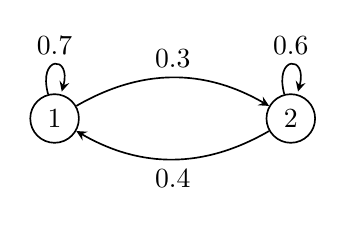
\begin{tikzpicture}[>=stealth, auto, semithick]

        % States
        \node[draw, circle] (A) at (0,0) {1};
        \node[draw, circle] (B) at (3,0) {2};

        % Transitions
        \draw[->] (A) to[bend left] node[above] {0.3} (B);
        \draw[->] (B) to[bend left] node[below] {0.4} (A);
        \draw[->] (A) edge[loop above] node {0.7} (A);
        \draw[->] (B) edge[loop above] node {0.6} (B);

    \end{tikzpicture}
    \caption[{
        Simple Markov chain schematic
    }]{
        A simple time-homogeneous Markov chain, with two states.
        It is characterised by the transition kernel
        $K(1, 1) = \Pr(X_{i + 1} = 1 | X_i = 1) = 0.7,$
        $K(1, 2) = \Pr(X_{i + 1} = 2 | X_i = 1) = 0.3,$
        $K(2, 1) = \Pr(X_{i + 1} = 1 | X_i = 2) = 0.4,$ and
        $K(2, 2) = \Pr(X_{i + 1} = 2 | X_i = 2) = 0.6.$ The stationary
        distribution is $\pi(1) = 4/7$ and $\pi(2) = 3/7.$
    }
    \label{fig:MC}
\end{figure}

Markov chains are characterised by a transition kernel $K$ with
$$K(x_i, x_{i + 1}) := \Pr(X_{i + 1} = x_{i + 1} | X_i = x_{i + 1}),$$
where this probability is interpreted as a density for continuous random
variables. $K(1, 1)$ would therefore be the probability of transitioning
from state 1
to state 2 in a single discrete time step.

We will restrict our focus to time-homogeneous Markov chains where
if the value of $X_i$ is known to be $x$, the behaviour of the chain from this point on
will be identical to the behaviour of the chain from $X_j,$ if this is also
observed to be $x$.

\begin{definition}[Time-Homogeneous]
    A Markov chain is \bemph{time-homogeneous} if
    $$
        \{X_i, X_{i+1}, \dots, X_{i + n}\}
        \overset{d}{=} \{X_{i^\prime}, X_{i^\prime+1}, \dots, X_{i^\prime + n}\}
    $$
    for all $i, i^\prime, n \in \mathbb{N},$ given $X_i = x = X_{i^\prime}.$
\end{definition}

The Markov chain in Figure \ref{fig:MC} is time-homogeneous. It does not
matter how long it took to get into a state, the Markov chain will behave the
same from that point forward.

\begin{definition}[Stationary Distribution]
    A Markov chain has \bemph{stationary distribution} $\pi$ if for $X_i \sim \pi,$
    then $X_{i + 1} | X_i \sim \pi.$
\end{definition}

\begin{example}
    Given the Markov chain in Figure \ref{fig:MC}, the stationary distribution
    can be calculated by solving the simultaneous equations
    \begin{align*}
        K(1, 1) \times \pi(1)
        + K(2, 1) \times \pi(2) = 0.7 \times \pi(1)
        + 0.4 \times \pi(2) = & \, \pi(1) \\
        \pi(1) + \pi(2) =     & \, 1.
    \end{align*}
    Therefore, $\pi(1) = 4/7$ and $\pi(2) = 3/7.$
\end{example}

As stated earlier, to sample from a distribution $p(x),$ we construct a Markov
chain with this stationary distribution. A sufficient condition to know that
we have achieved this is if our chain satisfies the detailed balance
condition.

\begin{theorem}[Detailed balance condition]
    A Markov chain has stationary distribution $p(x),$ which it converges to
    independent of initialisation, if for all $x, x^\prime,$
    $$p(x)K(x, x^\prime) = p(x^\prime)K(x^\prime, x).$$
\end{theorem}

\begin{proof}
    More formally this requires the notions of recurrent, non-null,
    irreducible and aperiodic Markov chains which we do not discuss here. 
    For a full
    discussion and proof
    see \cite[Chapter 6]{robert_monte_2010}.
\end{proof}

\subsubsection*{Metropolis-Hastings}

The Metropolis-Hastings algorithm is one way of constructing a Markov
chain with stationary distribution equal to the target distribution $g.$
We choose a proposal distribution $q(x^\prime| x)$ which given our last sample
$x,$ generates a new random
variable $X^\prime.$ For example $q$ might be the density of
$X^\prime \sim N(x, 1),$ a normal random variable with mean
around the previous sample. Then similar to rejection sampling, $X^\prime$
is accepted as the next state in the distribution with some probability
$\alpha$, chosen in such a way that if the chain is distributed according to
a stationary distribution
$X_i \sim g,$ then the next step will also be distributed according to that
stationary distribution $X_{i + 1}\sim g.$ Formally this is set out in
Algorithm \ref{alg:MH}.

\begin{algorithm}[htbp]
    \caption{Metropolis-Hastings Sampler}
    \label{alg:MH}
    \begin{algorithmic}
        \State Initialise $x_0$
        \For{$i = 1$ to $N$}
        \State Sample $X^\prime \sim q(x^\prime|x_{i - 1})$
        \State Compute acceptance ratio
        $\alpha
            = \min\left(
            \frac{
            g(x^\prime) q(x_{i - 1}|x^\prime)
            }{
            g(x_{i - 1}) q(x^\prime|x_{i - 1})
            },
            1
            \right)$
        \State Sample $U \sim \text{Uniform}(0, 1)$
        \If{$U \leq \alpha$}
        \State $x_i \gets X^\prime$
        \Else
        \State $x_i \gets x_{i-1}$
        \EndIf
        \EndFor
        \State \Return $\{x_0, x_1, \dots, x_N\}$
    \end{algorithmic}
\end{algorithm}

Note that for symmetric proposal distributions $q(x^\prime|x) = q(x|x^\prime),$
$\alpha$ simplifies to $\min\left(\frac{g(x^\prime)}{g(x)}, 1\right),$ in
which case the algorithm is simply called a Metropolis sampler.

\begin{theorem}
    The chain produced by Algorithm \ref{alg:MH}, $\{X_k\}_{k\in \mathbb{N}},$
    has stationary distribution $g$ for proposal distributions that cover the
    support of $g.$
\end{theorem}

\begin{proof}
    We show that the detailed balance condition
    $$
        g(x)q(x^\prime | x)\alpha(x, x^\prime)
        =g(x^\prime)q(x | x^\prime)\alpha(x^\prime, x)
    $$
    where $\alpha(x, x^\prime) = \min\left(
        \frac{
                g(x^\prime) q(x|x^\prime)
            }{
                g(x) q(x^\prime|x)
            },
        1
        \right)$
    is satisfied. Without loss of generality let
    $g(x^\prime) q(x|x^\prime) < g(x) q(x^\prime|x),$ so
    $\alpha(x, x^\prime) = \frac{
            g(x^\prime) q(x|x^\prime)
        }{
            g(x) q(x^\prime|x)
        },$ and $\alpha(x^\prime, x) = 1.$
    \begin{align*}
        g(x)q(x^\prime | x)\alpha(x, x^\prime)
        = & g(x)q(x^\prime | x) \times \frac{
            g(x^\prime) q(x|x^\prime)
        }{
            g(x) q(x^\prime|x)
        }                                                \\
        = & g(x^\prime) q(x|x^\prime)                    \\
        = & g(x^\prime) q(x|x^\prime)\alpha(x^\prime, x)
    \end{align*}
\end{proof}

\begin{figure}[htbp]
    \centering
    \includegraphics{coin_MH_R.pdf}
    \caption[{
        Metropolis-Hastings samples from the posterior distribution of $p,$ 
        for $y^\obs\sim\mathrm{Binom}(n, p)$
    }]{
        Samples from the posterior distribution of $p$ using the
        Metropolis-Hastings algorithm. $p$ was assumed to
        have a uniform prior between 0 and 1, with $y^\obs = 6,$ generated
        from $\mathrm{Binom}(10, p),$
        The choice of proposal distribution did not impact the final estimate
        of $\Pr(p | y^\obs).$
    }
    \label{fig:coin_R}
\end{figure}

As seen empirically in Example \ref{ex:coin_toss} and Figure \ref{fig:coin_R}, 
the proof does not depend on choice of proposal distribution.

\begin{example}[Coin toss]\label{ex:coin_toss}
    Let the probability of tossing heads on a weighted coin be
    $\Pr(X = 1) = p.$ Assume that $p\sim \mathrm{Unif}(0,1).$
    We observe $y^\obs = 6$ heads from 10 tosses of the coin.
    Therefore
    $$
        \Pr(p | y^\obs) \propto \Pr(y^\obs| p)\Pr(p)
        = \binom{n}{y^\obs}p^{y^\obs}(1 - p)^{n - y^\obs}\times 1
        = 210p^6(1-p)^4.
    $$
    We sample from this distribution using the Metropolis algorithm which
    becomes
    \begin{algorithmic}
        \State Initialise $p_0$
        \For{$i = 1$ to $N$}
        \State Sample $P^\prime \sim q(p^\prime|p_{i - 1})$
        \State Compute acceptance ratio
        $\alpha
            = \min\left(
            \frac{(P^\prime)^6(1-P^\prime)^4}{p_{i - 1}^6(1-p_{i - 1})^4}, 1
            \right)$ \Comment{Assuming $q$ symmetric}
        \State Sample $U \sim \text{Uniform}(0, 1)$
        \If{$U \leq \alpha$}
        \State $p_i \gets X^\prime$
        \Else
        \State $p_i \gets x_{i - 1}$
        \EndIf
        \EndFor
        \State \Return $\{p_0, p_1, \dots, p_N\}$
    \end{algorithmic}

    We can compare two
    different proposal distributions for $q(p^\prime | p)$,
    $P^\prime \sim N(p, 1/12),$ and
    the second being $P^\prime \sim \mathrm{Unif}(p - 1/2, p + 1/2).$ The first
    1000 samples were discarded as burn in, and it was thinned to every 5
    samples.
    The resulting distribution of the samples can be seen in Figure
    \ref{fig:coin_R}, with both proposal distributions resulting in samples
    that are good at estimating the true distribution.
\end{example}

Since the chain converges to the stationary distribution over time, and is
highly correlated,
a derived chain $\{x_{B + iT}\}_{i \in \mathbb{N}}$ is constructed
from the output. The
first $B$ samples are discarded as `burn in' samples to reduce the impact
of the initialisation point. The chain is `thinned' by taking every $T$th sample,
since $X_i$ and $X_{i + 1}$ may also be highly correlated (in samples where
the proposed $X^\prime$ is rejected, $X_i = X_{i + 1}$).
This derived chain is considered a
random sample from the target distribution $g.$
In practice, diagnostics such as trace plots and autocorrelation plots are used
to determine $B$ and $T$ (see
\cite[Chapter 11]{gelman_bayesian_2014}).

\begin{figure}[htbp]
    \centering
    \includegraphics[width=\textwidth]{SIS_beta_pred.pdf}
    \caption[{
        Metropolis-Hastings samples from the posterior distribution of $\beta$
        in an $SIS$ model given incidence data
    }]{
        Given a daily incidence of $y^\obs = 26$ at day 30 of an $SIS$ epidemic,
        with unknown $\beta,$ we use Metropolis-Hasting to
        sample from $\Pr(\beta | y^\obs).$
        $\gamma = 1/4$ was assumed to be correct, and we compared the assumption
        $y^\obs
            \sim \mathrm{Binom}(\lfloor S_{30} \rfloor,\, \beta I_{30}/N),$
        to the assumption $y^\obs \sim \Pois(\frac{\beta I_{30} S_{30}}{N})$
        where $I_{30}, S_{30}$ are the ODE solutions to Equations
        \ref{eq:SIS_1} and \ref{eq:SIS_2}. We assumed the prior distribution
        $\beta\sim \mathrm{Gamma}(2, 6),$ where $\E(\beta) = 1/3.$ Our proposal
        density was $N(\beta^\ast, 1/10),$ where $\beta^\ast$ was the previous
        sample.
    }
    \label{fig:SIS_MH_R}
\end{figure}

For disease models, given a prior distribution for the parameter(s) $\btheta,$
Metropolis-Hastings can be used to produce samples from
$\Pr(\btheta | y^\obs) \propto \mathcal{L}(\btheta)\Pr(\btheta),$ where
$\mathcal{L}(\btheta)\Pr(\btheta)$ can be calculated to a proportionality
constant but not directly
sampled from. For example given an $SIS$ model described in Equations
\ref{eq:SIS_1} and \ref{eq:SIS_2} with unknown effective contact rate
$\beta \sim \mathrm{Gamma}(2, 6)$ and daily case counts $y^\obs,$ we can
draw samples from $\btheta | y^\obs$ as in Figure \ref{fig:SIS_MH_R}. This
figure demonstrates that the choice of likelihood results in different posterior
sample distributions. The samples from Poisson likelihood have greater variance
than the samples from the binomial likelihood.

\subsubsection*{Gibbs Sampling}

\begin{algorithm}[htbp]
    \caption{Gibbs Sampler}
    \label{alg:gibbs}
    \begin{algorithmic}
        \State Initialise
        $\btheta^{(0)} = (\theta_1^{(0)}, \theta_2^{(0)}, \dots, \theta_d^{(0)})$
        \For{$i = 1$ to $N$}
        \State Sample
        $\theta_1^{(i)}
            \sim \Pr(
            \theta_1
            | \theta_2^{(i-1)}, \theta_3^{(i-1)}, \dots, \theta_d^{(i-1)}
            )$
        \State Sample
        $\theta_2^{(i)}
            \sim \Pr(
            \theta_2
            | \theta_1^{(i)}, \theta_3^{(i-1)}, \dots, \theta_d^{(i-1)})$
        \State $\vdots$
        \State Sample
        $\theta_d^{(i)}
            \sim \Pr(
            \theta_d
            | \theta_1^{(i)}, \theta_2^{(i)}, \dots, \theta_{d-1}^{(i)})$
        \State Save $(\theta_1^{(i)}, \theta_2^{(i)}, \dots, \theta_d^{(i)})$
        as $\btheta^{(i)}$
        \EndFor
        \State \Return $\{\btheta^{(0)}, \btheta^{(1)}, \dots, \btheta^{(N)}\}$
    \end{algorithmic}
\end{algorithm}

Some models may be structured such that it is possible
to sample from the parameters distributions 
$\theta_1 | \theta_2, \by^\obs$, and
$\theta_2 | \theta_1, \by^\obs$ but not the joint distribution of
$(\theta_1, \theta_2)| \by^\obs.$ A (multidimensional) Markov chain can be
constructed by iteratively updating the parameters. Such a method is called
a Gibbs sampler, described in
Algorithm \ref{alg:gibbs}. The distribution of the Markov chain
sampler will eventually converge to the
$\Pr(\theta_1, \theta_2 | \by^\obs),$ and for the same reasons as for
the Metropolis-Hastings
sampler, after thinning and discarding burn in, we consider the resulting
chain a sequence of independent samples from our target distribution.

\begin{theorem}[Gibbs Sampler]
    The Markov chain generated by Algorithm \ref{alg:gibbs}
    converges to the distribution of $\Pr(\btheta|\by^\obs).$
\end{theorem}

\begin{proof}
    We prove that the Gibbs Sampler satisfies the detailed balance
    equation for two unknown parameters.
    The transition kernel of the Markov chain is
    $$
        q(\btheta^{(i)}|\btheta^{(i-1)})
        := \Pr(\theta^{(i)}_1 | \theta^{(i-1)}_2, \by)
        \Pr(\theta^{(i)}_2 | \theta^{(i)}_1, \by).
    $$

    To prove the detailed balance condition is satisfied, we need to show that
    $$
        \Pr(\btheta^{(i-1)}| \by)q(\btheta^{(i)}|\btheta^{(i-1)})
        = \Pr(\btheta^{(i)}| \by)q(\btheta^{(i - 1)}|\btheta^{(i)}).
    $$

    \begin{align*}
        \Pr(\btheta^{(t-1)}| \by)q(\btheta^{(i)}|\btheta^{(i-1)})
        = & \, \Pr(\theta_1^{(i-1)}, \theta_2^{(i-1)}| \by) \times
        \Pr(\theta^{(i)}_1 | \theta^{(i-1)}_2, \by) \times
        \Pr(\theta^{(i)}_2 | \theta^{(i)}_1, \by)                        \\
        = & \, \Pr(\theta_1^{(i-1)}| \theta_2^{(i-1)}, \by) \times
        \Pr(\theta_2^{(i-1)}| \by) \times
        \Pr(\theta^{(i)}_1 | \theta^{(i-1)}_2, \by) \times
        \Pr(\theta^{(i)}_2 | \theta^{(i)}_1, \by)                        \\
        = & \, \Pr(\theta_1^{(i-1)}| \theta_2^{(i-1)}, \by) \times
        \Pr(\theta^{(i)}_1, \theta^{(i-1)}_2 | \by) \times
        \Pr(\theta^{(i)}_2 | \theta^{(i)}_1, \by)                        \\
        = & \, \Pr(\theta^{(i)}_2 | \theta^{(i)}_1, \by) \times
        \Pr(\theta^{(i)}_1, \theta^{(i-1)}_2 | \by) \times
        \Pr(\theta_1^{(i-1)}| \theta_2^{(i-1)}, \by)                     \\
        = & \, \Pr(\theta^{(i)}_2 | \theta^{(i)}_1, \by) \times
        \Pr(\theta^{(i)}_1 | \by)  \times
        \Pr(\theta^{(i-1)}_2 | \theta^{(i)}_1, \by) \times
        \Pr(\theta_1^{(i-1)}| \theta_2^{(i-1)}, \by)                     \\
        = & \, \Pr(\theta^{(i)}_1, \theta^{(i)}_2| \by) \times
        \Pr(\theta^{(i-1)}_2 | \theta^{(i)}_1, \by) \times
        \Pr(\theta_1^{(i-1)}| \theta_2^{(i-1)}, \by)                     \\
        = & \, \Pr(\btheta^{(t)}| \by) q(\btheta^{(i -1)}|\btheta^{(i)})
    \end{align*}
    as required, so the posterior distribution $\Pr(\btheta|\by)$ is the unique
    stationary distribution associated with the generated Markov chain.
\end{proof}

\begin{figure}[htbp]
    \centering
    \includegraphics{SIS_gibbs.pdf}
    \caption[{
        Gibbs samples from the joint posterior distribution of $\gamma$ and 
        $\beta$ in an $SIS$ model given an estimated $R_0.$
    }]{
        2000 posterior samples from $\Pr(\beta, \gamma | \by^\obs),$ where
        $\beta|\gamma, \by^\obs
            \sim \mathrm{Gamma}(9, 4/\gamma + 4 + 8\gamma)$ and
        $\gamma|\beta, \by^\obs
            \sim \mathrm{InvGamma}(12, 12\beta).$ The samples were
        obtained using a Gibbs sampler.
        The red points are the first 15 samples using the Gibbs sampler.
    }
    \label{fig:gibbs_R}
\end{figure}

\begin{example}
    Consider the $SIS$ model described by Equations \ref{eq:SIS_1}
    and \ref{eq:SIS_2}. Early in an epidemic, the average number of new
    cases generated from a single infectious individual is known as $R_0.$
    This can be shown to be $\frac{\beta}{\gamma}$ for the $SIS$ model.
    Let $\by^\obs = \{1, 1, 3, 1\}$ be the number of people infected by four
    different individuals at the start of the epidemic. We assume that the
    number of infections are generated from a Poisson distribution with mean
    $\frac{\beta}{\gamma}.$ Therefore, the likelihood is
    $$
        \mathcal{L}(\beta, \gamma):= \Pr(\by^\obs | \beta, \gamma)
        = \frac{
            \left(\frac{\beta}{\gamma}\right)^{1 + 1 + 3 + 1}
            \exp( -\frac{4\beta}{\gamma})
        }{
            1!\times 1! \times 3! \times 1!
        }
        \propto\left(\frac{\beta}{\gamma}\right)^{6}\exp( -\frac{4\beta}{\gamma}).
    $$
    Let us assume that from similar previous epidemics we know that
    $\beta | \gamma \sim \mathrm{Gamma}(3, 4 + 8\gamma),$ and
    $\gamma | \beta \sim \mathrm{InvGamma}(6, 8\beta).$ Therefore
    \begin{align*}
        \Pr(\beta|\gamma, \by^\obs)
        \propto & \Pr(\by^\obs|\gamma, \beta)\Pr(\beta|\gamma)      \\
        \propto &
        \left(\frac{\beta}{\gamma}\right)^{6}
        \exp( -\frac{4\beta}{\gamma})
        \times \beta^{3 - 1}\exp(-(4 + 8\gamma)\beta)               \\
        \propto & \beta^{9 - 1}\exp(-(4/\gamma + 4 + 8\gamma)\beta),
    \end{align*}
    and so
    $\beta|\gamma, \by^\obs
        \sim \mathrm{Gamma}(9, 4/\gamma + 4 + 8\gamma).$
    Similarly,
    \begin{align*}
        \Pr(\gamma|\beta, \by^\obs)
        \propto & \Pr(\by^\obs|\gamma, \beta)\Pr(\gamma|\beta)         \\
        \propto &
        \left(\frac{\beta}{\gamma}\right)^{6}
        \exp( -\frac{4\beta}{\gamma})
        \times \gamma^{- 6 - 1}\exp\left(-\frac{8\beta}{\gamma}\right) \\
        \propto & \gamma^{- 12 - 1}
        \exp\left(-\frac{12\beta}{\gamma}\right),
    \end{align*}
    and so
    $\gamma|\beta, \by^\obs
        \sim \mathrm{InvGamma}(12, 12\beta).$
    Now we have explicit forms for the conditional probabilities,
    we generate samples using the Gibbs sampler in Algorithm \ref{alg:gibbs}.
    Samples from the distribution can be seen in Figure \ref{fig:gibbs_R}.
\end{example}

The Gibbs sampler and Metropolis-Hastings sampler are often combined, by
using a Metropolis-Hastings sampler for each step of the conditional sampling.
This is useful when the conditional distributions
$\Pr(\theta_1 | \theta_2, \by^\obs)$ can be calculated up to a proportionality
constant, but not directly sampled from.

\subsection*{Approximate Bayesian Computation}

So far, under a Bayesian framework, parameter estimation has still been
dependent on the likelihood function
$\mathcal{L}(\btheta) := \Pr(\by^\obs|\btheta)$ through Bayes' theorem.
In many cases, such as stochastic disease models and agent based models, the
likelihood has no explicit form, or is intractable to calculate.
The only option here is to run the model given $\btheta,$
and sample $\by(\btheta)$ directly.

\begin{algorithm}[htbp]
    \caption{Naive Bayesian Sampler}
    \label{alg:naive_samp}
    \begin{algorithmic}
        \State Sample $\btheta^\ast \sim \Pr(\btheta)$
        \State Run model and compute $\by(\btheta^\ast)$
        \If{$\by(\btheta^\ast) = \by^\obs$}
        \State \Return $\btheta^\ast$ as a sample from $\Pr(\btheta|\by^\obs.)$
        \EndIf
    \end{algorithmic}
\end{algorithm}

Algorithm \ref{alg:naive_samp} outlines a naive method of using such model
runs to sample from
$\Pr(\btheta|\by^\obs)$ is to sample
$\btheta^\ast$ from $\Pr(\btheta),$ and run the model to obtain
$\by(\btheta^\ast).$ For each iteration,
$\by(\btheta^\ast)$ will exactly equal $\by^\obs$
with probability $\Pr(\by^\obs|\btheta^\ast)\Pr(\btheta^\ast)
    \propto \Pr(\btheta^\ast|\by^\obs),$
and hence if $\by(\btheta^\ast) = \by^\obs$ we can accept $\btheta^\ast$ 
as a sample
from our posterior parameter distribution. When
$\by^\obs|\btheta^\ast$ does not have a countable number of non-zero
probability outputs,
$\by(\btheta^\ast) = \by^\obs$ can be exactly zero, and even in the
countable case, for
higher dimensional $\by(\btheta),$ the probability of returning exactly
$\by^\obs$ vanishes. Therefore, we draw inspiration from the continuous
interpretation of the likelihood
$\mathcal{L}(\btheta) := \Pr(\by(\btheta) \in \diff \by^\obs|\btheta).$
Since

\begin{equation}\label{eq:dens_ball}
    \Pr(\by(\btheta) \in \diff \by^\obs|\btheta)
    := \lim_{\epsilon \to 0}
    \frac{\Pr(\by(\btheta) \in B^D_\epsilon(\by^\obs))}{\varepsilon},
\end{equation}

where $B^D_\epsilon(\by^\obs)$ is a ball of size $\epsilon$ around $\by^\obs,$
with respect to some (unknown) metric $D$ induced by the (unknown)
probability distribution of $\by(\btheta).$ Therefore, $\mathcal{L}(\btheta)$ is
approximately proportional
to $\Pr(\by(\btheta) \in B^D_\epsilon(\by^\obs) | \btheta),$
(as a function of $\btheta$).

Hence we construct a new approximate sampling algorithm where rather than
rejecting the sample for $\by(\btheta) \neq \by^\obs,$ we accept
$\by(\btheta)$ if it falls within a ball of size $\epsilon$ around $\by^\obs.$
Equivalently we accept samples if $D(\by(\btheta), \by^\obs) < \epsilon.$

Since the distribution of $\by(\btheta)$ is unknown, and since the metric
required for Equation \ref{eq:dens_ball} to hold depends on $\btheta,$ we do
not explicitly derive $D(\by(\btheta), \by^\obs),$ we are forced to
approximate it with $\tilde{D}(\by(\btheta), \by^\obs)$. The most common choice
of $\tilde{D}$ is the $L^p$ norm of $\by(\btheta) - \by^\obs$
$$
    \tilde{D}(\by(\btheta), \by^\obs)
    =||\by(\btheta) - \by^\obs||_p
    = \left(\sum_{i = 1}^d
    \left|y_i(\btheta)
    - y_i^\obs\right|^p\right)^{1/p},
$$
for $p\geq 1.$ For $p=1$ or $2$ this is the Manhattan or Euclidean distance
between the two vectors. When the observations in $\by^\obs$ are on different
scales, or $\by^\obs$ are highly correlated between model runs, care needs to
be taken to rescale $\by^\obs$ and $\by(\btheta)$ by a covariance matrix to
remove correlation, or by rescaling using the relative differences instead of
$||\by(\btheta) - \by^\obs||_p.$

\begin{algorithm}[htbp]
    \caption{Approximate Bayesian Computation Sampler}
    \label{alg:abc}
    \begin{algorithmic}
        \State Sample $\btheta^\ast \sim \Pr(\btheta)$
        \State Run model and compute $\mathcal{D}(\btheta^\ast)$
        \If{$\mathcal{D}(\btheta^\ast) < \epsilon$}
        \State \Return $\btheta^\ast$ as a sample from $\Pr(\btheta|\by^\obs.)$
        \EndIf
    \end{algorithmic}
\end{algorithm}

The full procedure is outlined in Algorithm \ref{alg:abc}, but since 
$\by^\obs$ is fixed, we consider $\tilde{D}(\by(\btheta), \by^\obs)$ as a
function of $\btheta,$ and
we can equivalently write 
$\mathcal{D}(\btheta) := \tilde{D}(\by(\btheta), \by^\obs).$
We call $\mathcal{D}(\btheta)$ the discrepancy function where in a
non-deterministic model, $\mathcal{D}(\btheta)$ is random.